\section{Auswertung}
\label{sec:Auswertung}
Im Folgenden wird der Versuch ausgewertet.\\
Die Messerte werden immer im Abstand von $\Delta t = \SI{1}{\minute}$ aufgenommen.
Die Reservoire werden jeweils mit genau abgemessenen $\SI{4}{\litre}$ Wasser befüllt.
Die Temperaturen werden auf 0,1 $ \si{\celsius} $ genau gemessen.
Die Druckskala von $ p_b $ kann auf $ \SI{0,1}{\bar} $ genau ablesen werden, die von $ p_a $ auf $ \SI{0,2}{\bar} $.
Die Kompressorleistung wird auf $ \SI{1}{\watt} $ genau bestimmt.
\subsection{Bestimmung einer Ausgleichskurve}
\begin{figure}[H]
  \centering
  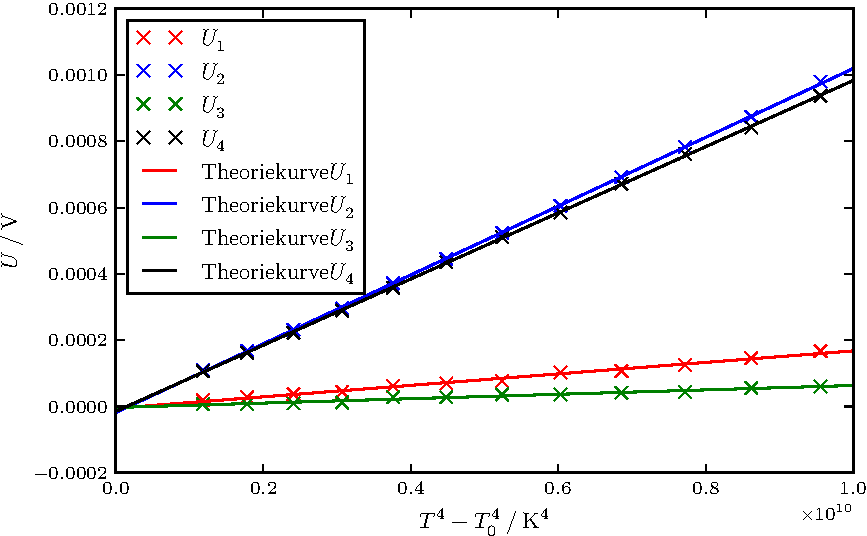
\includegraphics{plot.pdf}
  \caption{Temperaturverlauf.}
  \label{fig:plot}
\end{figure}
Die gemessenen Daten für die Temperatur $T_1$ des wärmeren sowie die Temperatur
$T_2$ des kälteren Reservoirs werden gegen die Zeit $t$ in Sekunden abgetragen.
Zum Plotten in Python wird Matplotlib benutzt, die Ausgleichsrechnung wird mit SciPy durchgeführt.
Für folgende Funktion wird das Ausgleichspolynom bestimmt:
\begin{equation}
  T(t)=A \cdot t^2 + B \cdot t + C
\end{equation}
Die Parameter $A$, $B$ und $C$ ergeben sich zu
\begin{align*}
A_{T_1} &= \SI[per-mode=fraction]{-3.9 +- 0.1e-6}{\kelvin\per\second²} \\
B_{T_1} &= \phantom{1}\SI[per-mode=fraction]{0.0234 +- 0.0002}{\kelvin\per\second} \\
C_{T_1} &= \phantom{1}\SI[per-mode=fraction]{293.29 +- 0.06}{\kelvin} \\
A_{T_2} &= \phantom{1}\SI[per-mode=fraction]{4.35 +- 0.09e-6}{\kelvin\per\second²}  \\
 B_{T_2} &= \SI[per-mode=fraction]{-0.0182 +- 0.0002}{\kelvin\per\second} \\
  C_{T_2} &= \phantom{1}\SI[per-mode=fraction]{294.94 +- 0.06}{\kelvin}
\end{align*}

Durch Ableiten und Einsetzen in die Ausgleichskurve
\begin{equation}
  \frac{\symup{d}T}{\symup{d}t}= 2 \cdot A \cdot t + B
\end{equation}
ergeben sich die Werte der Differentialquotienten, welche der Tabelle \ref{tab:tabelle1} entnommen werden können.
\\
Für die Fehlerrechnung wird bei der vorliegenden Rechnung und bei allen folgenden Rechnungen das Gaußsche Fehlerfortpflanzungsgesetz
\begin{equation}
\increment{f} = \sqrt{\Bigl(\frac{\partial f}{\partial x_1}\increment{x_1}\Bigr)^2 + \Bigl(\frac{\partial f}{\partial x_2}\increment{x_2}\Bigr)^2 + \dotsc + \Bigl(\frac{\partial f}{\partial x_n}\increment{x_n}\Bigr)^2}
\end{equation}
für eine Funktion $f(x_1,x_2, \dotsc ,x_n)$, bei der die Größen $x_1, x_2, \dotsc , x_n$ voneinander unabhängig sind, verwendet.
Dementsprechend beträgt der Fehler für die Differentialquotienten
\begin{equation}
  \Delta \frac{\symup{d}T}{\symup{d}t} = \sqrt{\Bigl(2\ \cdot A \cdot \Delta A \Bigr)^2 - \Bigl( \Delta T \Bigr)^2 }.
\end{equation}
Uncertainties hat jene und folgende Rechnungen übernommen.
\begin{table}
  \centering
  \caption{Differentialquotienten}
  \label{tab:tabelle1}
  \sisetup{table-format=1.2}
  \begin{tabular}{c c c c c}
    \toprule
    {$t [\si{\second}]$} & {$T_1 [\si{\kelvin}]$} & {$T_2 [\si{\kelvin}]$} & {$\frac{\symup{d}T_1}{\symup{d}t} [\si[per-mode=fraction]{\kelvin\per\second}]$}  & {$\frac{\symup{d}T_2}{\symup{d}t} [\si[per-mode=fraction]{\kelvin\per\second}]$}\\
    \midrule
    \num{420} & \num{29.6 +- 0.1} & \num{14.9 +- 0.1} & \num{0.02020 +- 0.0002} & \num{-0.0145 +- 0.0002} \\
    \num{840} & \num{37.5 +- 0.1} & \num{19.5 +- 0.1} & \num{0.01694 +- 0.0003} & \num{-0.0108 +- 0.0002} \\
    \num{1260} & \num{43.7 +- 0.1} & \num{5.7 +- 0.1} & \num{0.01368 +- 0.0003} & \num{-0.0071 +- 0.0003} \\
    \num{1680} & \num{48.9 +- 0.1} & \num{3.5 +- 0.1} & \num{0.01043 +- 0.0004} & \num{-0.0040 +- 0.0003} \\
    \bottomrule
  \end{tabular}
\end{table}
\subsection{Güteziffervergleich}
Für eine ideale Wärmepumpe gilt
\begin{equation}
  v_{ideal} = \frac{T_1}{T_1-T_2}.
\end{equation}
Für die reale Wärmepumpe gilt jedoch die Formel
\begin{equation}
  v_{real}= \frac{\symup{d} Q_1}{\symup{d} tN} = (m_1c_w+m_kc_k)\frac{\symup{d} T_1}{\symup{d} tN}.
\end{equation}
wobei $ N$ die Kompressorleistung, $ m_1$ die Masse des Wassers in $ R_1 $, $m_k$ die Masse des zu heizenden Reservoirs inklusive Kupferrohre, $ c_w $ die spezifische Wärmekapazität des Wassers sowie $ c_k $ die spezifische Wärmekapazität des Reservoirs und der Kupferrohre ist.
Es werden folgende Werte benutzt:
\begin{align*}
  \rho_{H_2O} &= \SI[per-mode=fraction]{0.998}{\gram\per\centi\metre\tothe{3}} \\
  m_1 = \rho{H_2O} \cdot V &= \SI[per-mode=fraction]{3,992}{\kilogram} \\
  m_k \cdot c_k &= \SI[per-mode=fraction]{750}{\joule\per\kelvin} \\
  c_w &= \SI[per-mode=fraction]{4184}{\joule\per\kilogram\per\kelvin} \\
\end{align*}
 \cite{lecher2001taschenbuch} \\
Die Kompressorleistung ergibt sich aus dem arithmetischen Mittelwert der Messdaten zu $N=\SI{124.8+-1.1}{\watt}$.
Für die Differentialquotienten wurden die Werte der Ausgleichskurve, angegeben in Tabelle 1, verwendet.
Es ergeben sich nach der Gaußschen Fehlerfortpflanzung die Fehlerformeln
\begin{equation}
  \Delta v_{\text{ideal}} = \sqrt{ \Bigl( \frac{-T_2}{(T_1-T_2)^2} \Delta T_1 \Bigr)^2 + \Bigl( \frac{T_1}{(T_1-T_2)^2} \Delta T_2 \Bigr)^2}
\end{equation}
sowie
\begin{equation}
  \Delta v_{\text{real}} = \sqrt{ \Bigl( (m_1 c_w + m_k c_k) \cdot \frac{1}{N} \cdot\Delta(\frac{\symup{T_1}}{\symup{d}t}   \Bigr)^2 + \Bigr( (m_1 c_w + m_k c_k) \cdot \frac{\symup{T_1}}{\symup{d}t} \cdot \frac{1}{N^2} \cdot \Delta N  \Bigl)^2 } .
\end{equation}
\begin{table}[H]
  \centering
  \caption{Güteziffervergleich.}
  \label{tab:tabelle2}
  \sisetup{table-format=1.2}
\begin{tabular}{c c c c c c}
  \toprule
  {$t [\si{\second}]$} & {$T_1 [\si{\kelvin}]$} & {$T_2 [\si{\kelvin}]$} & {$\increment{T} [\si{\kelvin}]$} & {$v_{real, T_1}$} & {$v_{ideal}$}\\
  \midrule
  \num{420} & \num{29.6 +- 0.1} & \num{14.9 +- 0.1} & \num{14.7 +- 0.1} & \num{2.83 +- 0.04} & \num{20.6 +- 0.2} \\
  \num{840} & \num{37.5 +- 0.1} & \num{19.5 +- 0.1} & \num{18.0 +- 0.1} & \num{2.37 +- 0.04} & \num{11.10 +- 0.05}  \\
  \num{1260} & \num{43.7 +- 0.1} & \num{5.7 +- 0.1} & \num{38.0 +- 0.1} & \num{1.91 +- 0.05} & \num{8.34 +- 0.03}  \\
  \num{1680} & \num{48.9 +- 0.1} & \num{3.5 +- 0.1} & \num{45.4 +- 0.1} & \num{1.46 +- 0.06} & \num{7.10 +- 0.02}  \\
  \bottomrule
\end{tabular}
\end{table}

\subsection{Massendurchsatz}
Bei einer Wärmepumpe wird dem kälteren Reservoir, hier $R_2$, die Wärmeenergie $Q_2$ in Form von Verdampfungswärme entzogen.
Der Zusammenhang zwischen dem Massendurchsatz $\frac{\symup{d} m}{\symup{d} t}$ und der entnommenen Wärmemenge pro Zeit $\frac{\symup{d} Q_2}{\symup{d} t}$ wird durch
\begin{equation}
  \frac{\symup{d} Q_2}{\symup{d}t} = L \cdot \frac{\symup{d} m}{\symup{d} t}
    \label{eqn:md}
\end{equation}
beschrieben, wobei $L$ die Verdampfungswärme des Mediums ist \cite{V203}.
Dabei gibt $L$ an, welche Energie pro Mol erforderlich ist, um einen Stoff bei gleichbleibender Temperatur zu verdampfen.
$L$ kann dabei der Dampfdruckkurve des jeweiligen Stoffes entnommen werden, welche den Phasenübergang zwischen flüssig und gasförmig in einem $pT$-Diagramm beschreibt.
Diese Kurve wird im Allgemeinen durch die Clausius-Clapeyronsche Gleichung beschrieben, aus der unter vereinfachten Bedingungen der Zusammenhang
\begin{equation}
  ln(p)= -\frac{L}{R}\frac{1}{T} + const
  \label{eqn:ccg}
\end{equation}
folgt.
Hierbei ist $R$ die allgemeine Gaskonstante.
Um nun den Wert von L für das genutzte Medium $\ce{Cl2F2C}$ zu bestimmen, wurden die Kehrwerte der Drucktemperaturen gegen den natürlichen Logarithmus des dazugehörigen Drucks abgetragen.
\begin{figure}[H]
  \centering
  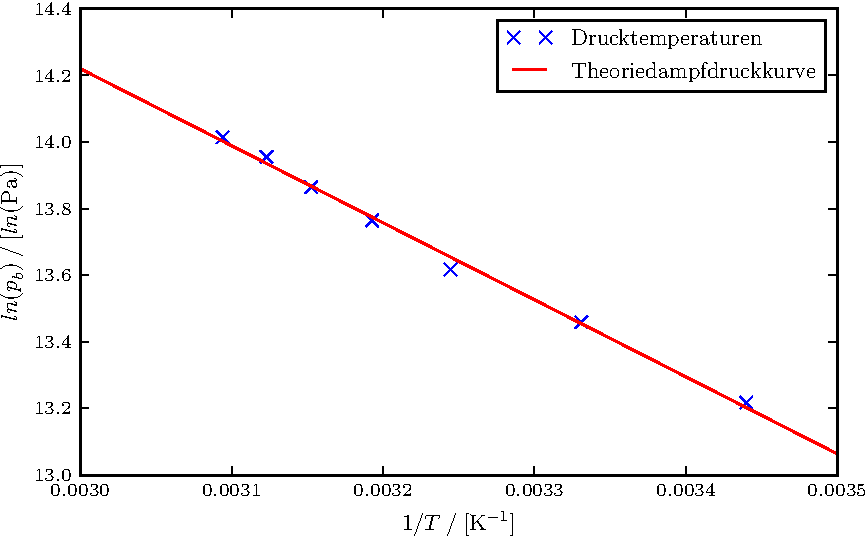
\includegraphics{plot2.pdf}
  \caption{Dampfdruckkurve.}
  \label{fig:plot2}
\end{figure}
Durch lineare Ausgleichsrechnung mit SciPy wurden die Parameter $b$ und $m$ der Ausgleichsgerade bestimmt zu:
\begin{align*}
m &= \SI{-2313.109 +- 70.380}{\kelvin} & b &= \num{21.160 +- 0.227}
\end{align*}
Aus dem bereits genannten Zusammenhang \eqref{eqn:ccg} ergibt sich die Verdampfungswärme $L$ nun zu
\begin{align*}
  L = -m \cdot R = \SI[per-mode=fraction]{19231.19 +- 572.47}{\joule\per\mol}.
\end{align*}
Aus dem allgemeinen Zusammenhang für die Verdampfungswärme \eqref{eqn:md} kann nun der Massendurchsatz bestimmt werden:

\begin{table}
  \centering
  \caption{Massendurchsatz.}
  \label{tab:tabelle3}
  \sisetup{table-format=1.2}
\begin{tabular}{c c c}
  \toprule
  {$t [\si{\second}]$} & {$T_2 [\si{\kelvin}]$} & {$\frac{\symup{d} m}{\symup{d} t} [\si{\mol\per\second}]$}\\
  \midrule
  \num{420} & \num{14.9 +- 0.1} & \num{0.013732 +- 0.00048} \\
  \num{840} & \num{19.5 +- 0.1} & \num{0.010274 +- 0.00039}\\
  \num{1260} & \num{5.7 +- 0.1} & \num{0.006814 +- 0.00034}  \\
  \num{1680} & \num{3.5 +- 0.1} & \num{0.003354 +- 0.00033} \\
  \bottomrule
\end{tabular}
\end{table}
\subsection{Kompressorleistung}
Um die Wärmemenge als Kondensationswärme an das Reservoir $R_1$ abgeben zu können, komprimiert der Kompressor $K$ das Gas, so dass es flüssig wird.
Da der Kompressor das Volumen $V_1$ bei einem Druck $p_b$ zum Volumen $V_2$ verringert, errechnet sich die verrichtete Arbeit zu
\begin{equation}
  W = - \int_{V_1}^{V_2} p_b \symup{d}V.
\end{equation}
Idealerweise findet dieser Prozess nahezu adiabatisch statt, so dass aus der Adiabatengleichung für die verrichtete Arbeit
\begin{equation}
  W = \frac{1}{\kappa -1}\Bigl(p_b \sqrt[\kappa]{\frac{p_a}{p_b}} - p_a \Bigr) V_a
\end{equation}
folgt.
Um die mechanische Kompressorleistung $P_{\text{mech}}$ zu bestimmen, wird der Quotient aus $\increment W$ und $\increment t$ gebildet.
Wird zudem das Volumen $V_a$ durch den Quotienten aus der Masse $m$ und der Dichte $\rho$ ersetzt, ergibt sich
\begin{equation}
  P_{\text{mech}} = \frac{1}{\kappa -1}\Bigl(p_b \sqrt[\kappa]{\frac{p_a}{p_b}} - p_a \Bigr) \frac{1}{\rho} \frac{\increment m}{\increment t} \cdot M \cdot 10^{-3}.
\end{equation}
$\kappa$ ist der Adiabatenkoeffizient des Mediums, für $\ce{Cl2F2C}$ durch $\kappa = 1.14$ gegeben, $p_a$ und $p_b$ die Drücke bei denen der Kompressor arbeitet, $\rho$ die Dichte des Gases unter $p_a$, $\frac{\increment m}{\increment t}$ der Massendurchsatz und $M$ die Molmasse des Mediums, für $\ce{Cl2F2C}$ durch $M = \SI{120.91}{\gram\per\mol}$ gegeben. Der Faktor $10^{-3}$ wurde ergänzt, um den Massendurchsatz in SI-Einheiten umzurechnen. \\
Um die Dichte $\rho$ zu bestimmen, wird die allgemeine Gasgleichung
\begin{equation}
  p V=m R_s T
\end{equation}
verwendet, $R_S$ ist die spezifische Gaskonstante. Diese bestimmt sich durch gegebenes $\rho_0=\SI{5,51}{\gram\per\litre}$ bei Normalbedingungen für das vorhandene Transportmedium zu $R_S = \SI{76.513}{\joule\per\kilogram\per\kelvin}$.\cite{sample}
Hieraus können die Dichten für alle Messzeitpunkte berechnet werden.
\begin{table}
  \centering
  \caption{Kompressorleistung.}
  \label{tab:tabelle4}
  \sisetup{table-format=1.2}
\begin{tabular}{c c c}
  \toprule
  {$t [\si{\second}]$} & {$\rho [\si{\gram\per\litre}]$} & {$P_{\text{mech}} [\si{\joule\per\second}]$}\\
  \midrule
  \num{420} & \num{19.961 +- 0.907} & \num{17.697 +- 1.736} \\
  \num{840} & \num{17.568 +- 0.925} & \num{22.014 +- 1.641} \\
  \num{1260} & \num{16.870 +- 0.937} & \num{17.809 +- 1.326} \\
  \num{1680} & \num{16.296 +- 0.945} & \num{10.143 +- 1.120} \\
  \bottomrule
\end{tabular}
\end{table}
